\documentclass{beamer}
\usepackage[utf8]{inputenc}   
\usepackage[T1]{fontenc}       
\usepackage[polish]{babel}     
\usepackage{pifont}
\setbeamertemplate{caption}{\insertcaption}
\usetheme{CambridgeUS}

\title{Jak gry komputerowe wpływają na dzieci?} %1slajd
\author{Daniel Szokało}
\date{19 stycznia, 2025}
\begin{document}
\begin{frame}
    \titlepage
\end{frame}

\begin{frame}{Plan prezentacji} %2slajd
\begin{itemize}
    \item[\ding{107}] Wstęp.
    \item[\ding{107}] Klasyfikacja gier komputerowych.
    \item[\ding{107}] Pozytywne aspekty grania w gry komputerowe.
    \item[\ding{107}] Negatywne skutki nadmiernego grania.
    \item[\ding{107}] Wnioski.
\end{itemize}
\end{frame}

\begin{frame}{Wstęp} %3slajd
\begin{columns}
% Column 1
\begin{column}{0.5\textwidth}
Gry komputerowe stały się powszechną formą rozrywki wśród dzieci. Z jednej strony, mogą one pobudzać kreatywność dzieci, kształtować relację, czy chociażby edukować. Z drugiej jednak, nadmierne granie, szczególnie w gry zawierające przemoc, może prowadzić do uzależnienia, problemów ze zdrowiem psychicznym, czy agresji. Jak znaleźć złoty środek?

\end{column}
% Column 2    
\begin{column}{0.5\textwidth}
    \begin{figure}
    \centering
        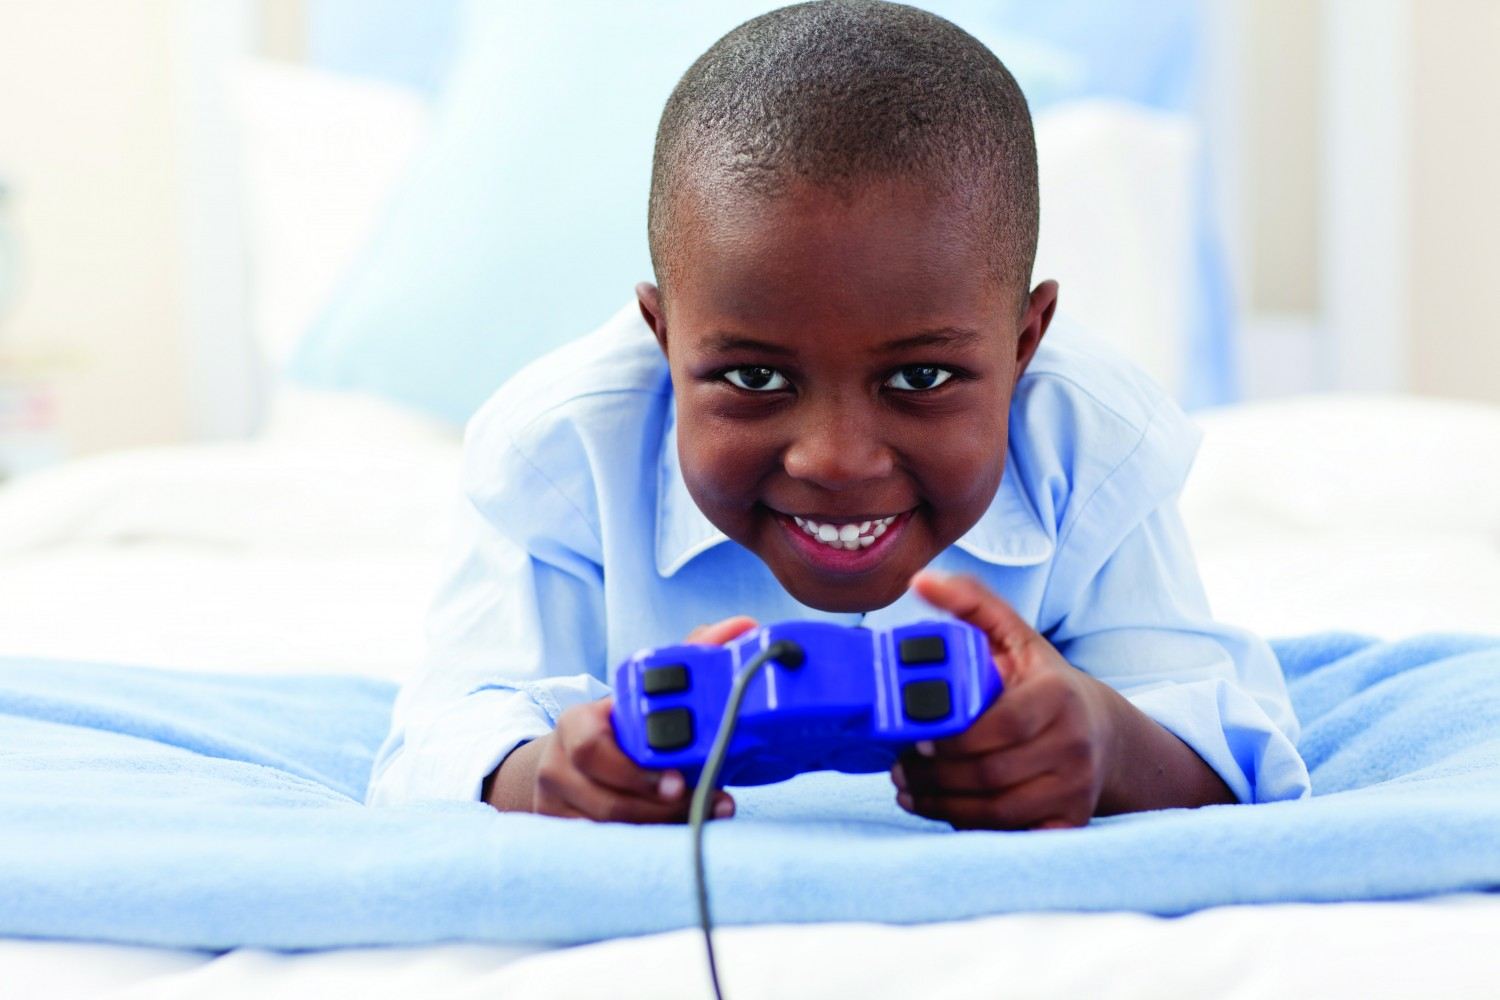
\includegraphics[width=6cm,height=4.5cm]{dziecko.jpg}
\end{figure}
\end{column}
\end{columns}
\end{frame}

\begin{frame}{Klasyfikacja gier komputerowych} %4slajd
 \small Gry komputerowe to prawdziwy kalejdoskop. Każdy typ posiada swój własny,
niepowtarzalny charakter i znacznie się od siebie różni. Wyróżnić możemy różne ich gatunki:

\begin{columns}
% Column 1
\begin{column}{0.5\textwidth}
        \normalsize \textbf {GRY FABULARNE (RPG)}
\newline
\small Gatunek gier komputerowych, w których gracz kontroluje stworzonego przez siebie bohatera. Cieszy się ogromną popularnością wśród graczy przez ową możliwość kontrolowania własnej postaci, rozwijania jej umiejętności przez zdobywanie doświadczenia i nagród, czy podejmowania trudnych decyzji. Przykładami takich tytułów może być The Witcher, Final Fantasy czy Minecraft.

\end{column}
% Column 2    
\begin{column}{0.5\textwidth}
    \begin{figure}
    \centering
        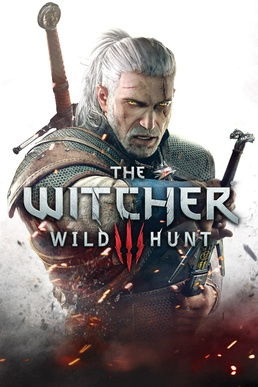
\includegraphics[width=4cm,height=5.5cm]{W3.jpg}
\end{figure}
\end{column}
\end{columns}
\end{frame}

\begin{frame} %5slajd
\begin{columns}
% Column 1
\begin{column}{0.5\textwidth}
    \begin{figure}
    \centering
        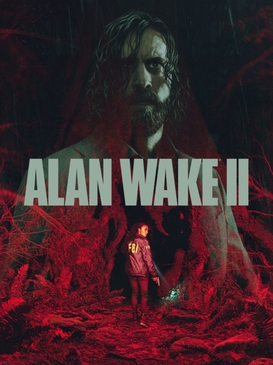
\includegraphics[width=5cm,height=6cm]{AW2.jpg}
\end{figure}
\end{column}

% Column 2
\begin{column}{0.5\textwidth}
	   \normalsize \textbf {GRY AKCJI}
\newline
 \small W grach akcji, oprócz momentów wymagających zręczności i błyskawicznych reakcji (często w walce lub w celu jej ominięcia), rozgrywka polega głównie na zbieraniu przedmiotów, eksploracji oraz rozwiązywaniu zagadek. Schemat często wygląda w następujący sposób: pokonujesz wrogów, przechodzisz poziomy, realizujesz misje. Kto nie zna Resident Evil, Alana Wake’a czy Silent Hill?
\end{column}
\end{columns}
\end{frame}

\begin{frame} %6slajd
\begin{columns}
% Column 1
\begin{column}{0.5\textwidth}
        \normalsize \textbf {GRY LOGICZNE}
\newline
\small To prawdziwe wyzwanie. Zmuszają nas do intensywnego myślenia i rozwiązywania trudnych zagadek. Planowanie, czy logiczne myślenie to jedynie przykładowe umiejętności jakimi musi posługiwać się gracz, który gra w tytuły takie jak Portal, Tetris czy Gwint: Wiedźmińska gra karciana.

\end{column}
% Column 2    
\begin{column}{0.5\textwidth}
    \begin{figure}
    \centering
        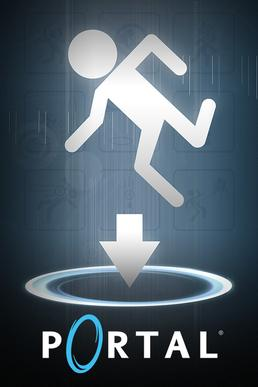
\includegraphics[width=4.5cm,height=6cm]{Portal.jpg}
\end{figure}
\end{column}
\end{columns}
\end{frame}

\begin{frame} %7slajd
\begin{columns}
% Column 1
\begin{column}{0.5\textwidth}
    \begin{figure}
    \centering
        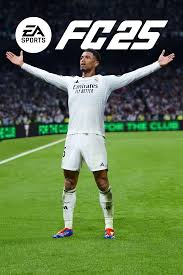
\includegraphics[width=4.5cm,height=6cm]{FC25.jpg}
\end{figure}
\end{column}

% Column 2
\begin{column}{0.5\textwidth}
	   \normalsize \textbf {GRY SPORTOWE}
\newline
 \small Są obowiązkową pozycją dla miłośników sportu. Charakteryzują się dużym wsparciem dla trybu wieloosobowego, aby mieć możliwość zmierzenia w piłce nożnej, koszykówce, tenisie, czy w wyścigach z innymi graczami lub znajomymi. Kto zdobędzie najwięcej punktów? A może marzysz o karierze sportowca i trybie dla jednego gracza? Tyle i jeszcze więcej czeka w grach takich jak EA Sports FC, NBA 2K i Gran Turismo. 

\end{column}
\end{columns}
\end{frame}

\begin{frame} %8slajd
\begin{columns}
% Column 1
\begin{column}{0.5\textwidth}
        \normalsize \textbf {GRY SYMULACYJNE}
\newline
\small To gatunek gier, które są stworzone po to, aby naśladować czynności, działania, które można zaobserwować w prawdziwym świecie. Celem tych gier może być nauczenie się czegoś lub po prostu wcielenie się w rolę, która nas interesuje (przykładowo w strażaka, gdzie wysyłani jesteśmy w samo centrum akcji ratowniczej). Przykładami takich gier może być seria gier The Sims czy Firefighting Simulator.

\end{column}
% Column 2    
\begin{column}{0.5\textwidth}
    \begin{figure}
    \centering
        
\includegraphics[width=6cm,height=3cm]{SIMS.png}
\end{figure}
\end{column}
\end{columns}
\end{frame}

\begin{frame} %9slajd
\begin{columns}
% Column 1
\begin{column}{0.5\textwidth}
    \begin{figure}
    \centering
        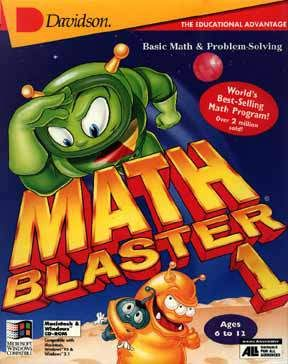
\includegraphics[width=5cm,height=6.5cm]{MB.jpg}
\end{figure}
\end{column}

% Column 2
\begin{column}{0.5\textwidth}
	   \normalsize \textbf {GRY EDUKACYJNE}
\newline
 \small Uczą gracza przez zabawę. Kto by pomyślał, że matematyka, języki, czy historia mogą być takie ekscytujące? Gry, takie jak Math Blaster czy City Car Driving, podnoszą naukę na jeszcze wyższy poziom. 

\end{column}
\end{columns}
\end{frame}

\begin{frame}{Pozytywne aspekty grania w gry komputerowe} %10slajd
Granie w gry komputerowe może przynieść wiele dobrego, pod warunkiem, że odbywa się z odpowiednim umiarem. Oto niektóre pozytywne aspekty, wynikające z grania: 
\newline

        \normalsize \textbf {Rozwój zdolności poznawcznych}
\newline
Gry komputerowe, zwłaszcza te, które stawiają przed graczem zagadki i wyzwania logiczne, potrafią rozwijać umysł młodego człowieka. Portal to nie tylko zabawa z przyjaciółmi, ale również cenna lekcja kooperacji z drugim człowiekiem. Znajomi uczą się analizować przeróżne sytuacje, podejmować trudne decyzje w mgnieniu oka i rozwiązywać zagadki. Kształtują swoją pamięć i zdolność skupienia. 

\end{frame}

\begin{frame} %11slajd
\begin{columns}
% Column 1
\begin{column}{0.5\textwidth}
	   \normalsize \textbf {Wzrost zdolności motorycznych}
\newline
 Gry wideo, głównie te z szybką, dynamiczną akcją (np. strzelanki) mogą wyostrzyć zmysł obserwacji, widzenie peryferyjne czy refleks. Gracze muszą cały czas monitorować ekran, rozpoznać szybko zmieniające się sytuacje, a następnie wykonać odpowiednią do sytuacji akcję.
\end{column}

% Column 2
\begin{column}{0.5\textwidth}
	   \normalsize \textbf {Zachęcenie do nauki}
\newline
 \small Nie od dziś wiadomo, że coraz to więcej firm decyduje się tworzyć gry, które nie tylko mają dostarczać zabawę młodym graczom, ale również ich czegoś nauczyć. Math Blaster to tylko jedna z takich gier, która pokazuje, że nie zawsze tradycyjna nauka jest najlepszym rozwiązaniem. Udowadnia, że łącząc naukę z elementami wirtualnymi można zapamiętać z nauki więcej, niż „normalnie” w tradycyjny sposób.

\end{column}
\end{columns}
\end{frame}

\begin{frame}{Negatywne skutki grania w gry komputerowe} %12slajd
Niestety, zbyt intensywne zanurzenie w świat gier może przynieść poważne konsekwencje dla zdrowia dzieci. Oto ich najważniejsza lista:
\newline

        \normalsize \textbf {Uzależnienie od gier}
\newline
Coraz więcej młodych osób spędzając czas przed monitorem traci poczucie czasu i nim się spojrzy, dzień się kończy. Częste takie przypadki mogą w końcu doprowadzić do niebezpiecznego zjawiska- uzależnienia. Gry kuszą na każdym kroku, a dzieci wciągają się bez reszty. Spędzają coraz więcej czasu w wirtualnym świecie, zaniedbując relacje z rodziną i rówieśnikami. 

\end{frame}

\begin{frame} %13slajd
\begin{columns}
% Column 1
\begin{column}{0.5\textwidth}
	   \normalsize \textbf {Problemy zdrowotne}
\newline
W parze z uzależnieniem idą problemy zdrowotne. Długotrwałe patrzenie na ekran prowadzić może do zmęczenia oczu, pogłębienia się ich wady, czy bólu głowy. Ponadto, spędzanie całego dnia bez żadnej aktywności fizycznej, jedząc niezdrowe jedzenie i pijąc gazowane napoje pogłębia problem otyłości, a siedzenie cały czas w jednej pozycji może prowadzić do problemów z kręgosłupem i chodzeniem.
\end{column}

% Column 2
\begin{column}{0.5\textwidth}
	   \normalsize \textbf {Problemy emocjonalne i społeczne}
\newline
 \small Negatywne skutki emocjonalne i społeczne grania w gry komputerowe przez dzieci mogą być bardzo różnorodne. Nadmierne granie, szczególnie w gry zawierające elementy przemocy i które oferują porównania z innymi graczami, może prowadzić do frustracji i poczucia niepowodzenia, co może wpłynąć na samoocenę dziecka, a także z izolacją społeczną, zaburzeniami komunikacyjnymi i trudnościami w relacjach z rówieśnikami. 

\end{column}
\end{columns}
\end{frame}

\begin{frame}{Wnioski} %14slajd
\begin{columns}
% Column 1
\begin{column}{0.5\textwidth}
Na zakończenie, co możemy wywnioskować? Gry komputerowe mają ogromny wpływ na rozwój dzieci i trzeba brać je z dużą dozą ostrożności. Z jednej strony, mogą rozwijać umysł, emocje, relacje międzyludzkie oraz motywować do nauki. Z drugiej jednak, nadmierne granie może zaszkodzić zdrowiu, psychice i prowadzić do nałogu. Aby korzystać z gier w sposób zdrowy, ważne jest, aby czas spędzany na grach był kontrolowany, a gry wybierane zgodnie z wiekiem dziecka i jego zainteresowaniami.

\end{column}
% Column 2    
\begin{column}{0.5\textwidth}
    \begin{figure}
    \centering
        
\includegraphics[width=6cm,height=5.5cm]{dziecko2.jpg}
\end{figure}
\end{column}
\end{columns}
\end{frame}

\begin{frame}%15slajd
		\frametitle{Bibliografia}
			\begin{thebibliography}{99}
			\bibitem{1}
			https://www.northeastohioparent.com/aging-stages/help-gamers-manage-screen-time/ 
			\bibitem{2}
			https://en.wikipedia.org/wiki/TheWitcher3:WildHunt 
                               \bibitem{3}
			https://en.wikipedia.org/wiki/AlanWake2 
			\bibitem{4}
			https://en.wikipedia.org/wiki/Portal(videogame) 
                                \bibitem{5}
			https://en.namu.wiki/w/EA
			\bibitem{6}
			https://pl.wikipedia.org/wiki/TheSims(seria) 
                                \bibitem{7}
			https://en.wikipedia.org/wiki/MathBlasterEpisodeI:InSearchofSpot 
                                \bibitem{8}
			https://ichtis.info/komputerowy-narkotyk/5820 
		\end{thebibliography}
	\end{frame}


\end{document}